%!TEX root = ../Thesis.tex

\chapter{Konzeption des Spurerkennung-Moduls}
\label{cha:konzeption}

In diesem Kapitel der Arbeit wird das zu entwickelnde Teilmodul \textit{``Spurerkennung''}
der MEC-View \textit{TrackerApplication} konzipiert. Hierzu wird zuerst dessen Rolle und Position im Gesamtkontext
der Anwendung betrachtet. Anschließend werden Anforderungen und ein Entwurf des Moduls aufgestellt.

Das Modul \textit{Spurerkennung} dient der Erreichung der in Abschnitt
\ref{sec:motivation_goals} definierten Ziele. Erstellt wird es im Rahmen des MEC-View Teilprojektes
\textit{Luftbeobachtung} als Teilmodul der Anwendung \textit{TrackerApplication}.
Abbildung \ref{fig:concept_laneDetection_context} gibt einen Überblick über das System.
Es werden hierbei jene Module beziehungsweise Schritte vorgestellt, welche mit der Spurerkennung in
Zusammenhang stehen.

\begin{figure}[H]
    \centering
    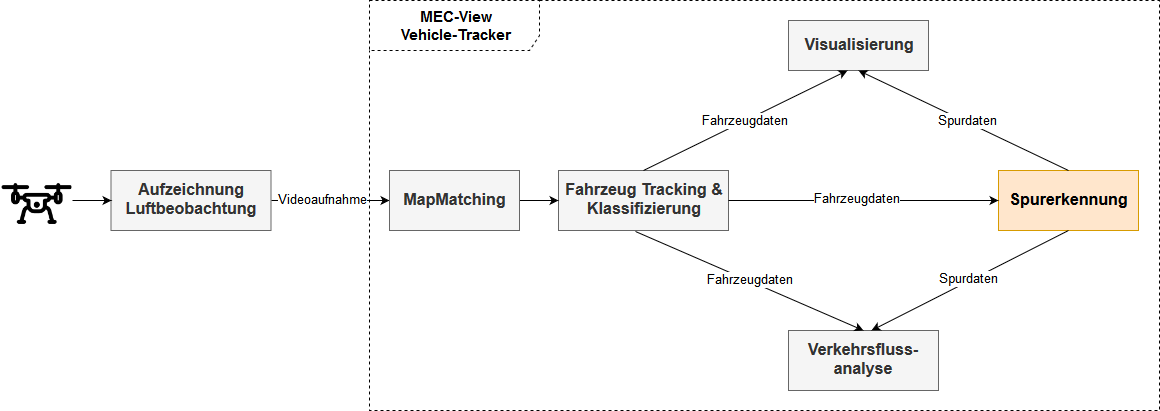
\includegraphics[width=\linewidth]{../resources/img/konzeption/Context_LaneDetection}
    \caption{Kontext des Spurerkennung Moduls}
    \label{fig:concept_laneDetection_context}
\end{figure}

Die mithilfe von Drohnen erstellten Videoaufnahmen können in der MEC-View \textit{TrackerApplication}
verarbeitet und analysiert werden. In einem ersten Schritt \textit{``MapMatching''}, wird hierzu üblicherweise
ein Welt-Koordinatensystem in Metern definiert. Anschließend können die Positionen und Typen
der Fahrzeuge bestimmt werden. Diese ersten zwei Schritte, welche der Extraktion von Fahrzeuginformationen
dienen, sind in Abschnitt \ref{sec:position_extraction} genauer beschrieben.
Die Fahrzeuginformationen, insbesondere die Positionsinformationen, dienen anschließend dem \textit{Spurerkennung}-Modul
als Eingabe. Aus ihnen extrahierte Spurdaten können anschließend in der Anwendung visualisiert werden oder in Kombination
mit den Fahrzeuginformationen zur Analyse des Verkehrsflusses eingesetzt werden.


\section{Anforderungen an das Modul}
\label{sec:requirements}
% Vorstellung er funk. und nicht-funk. Requirements an Modul

In diesem Abschnitt werden die wichtigsten funktionalen und nicht funktionalen Anforderungen
des Moduls festgehalten.

\subsection{Funktionale Anforderungen}

\paragraph{Anforderung 1000 (Top-Level)}
Das \textit{Spurerkennungs}-Modul soll es ermöglichen, mithilfe der \textit{TrackerApplication}
automatisch Fahrspuren aus den Positionsinformationen von Fahrzeugen in Luftaufnahmen abzuleiten.

\paragraph{Anforderung 2000}
Das Modul soll die Erkennung von Fahrspuren in den in Kapitel \ref{cha:street_topologies} vorgestellten
Straßentopologien unterstützen.

\paragraph{Anforderung 2100}
Das Modul soll unabhängig vom Aufnahmewinkel der Kamera Fahrspuren zuverlässig aus Videoaufnahmen ableiten können. 

\paragraph{Anforderung 2200}
Das Modul soll Fahrspuren bei Überlagerungen sinnvoll partitionieren können.

\paragraph{Anforderung 2300}
Das Modul soll die Enden benachbarter und paralleler Fahrspuren angleichen. Dies dient ihrer Verwendung in der
Verkehrsfluss-Analyse.

\paragraph{Anforderung 2400}
Das Modul soll es ermöglichen, die aus den Trajektorien abgeleiteten Fahrspuren in der \textit{TrackingApplication}
zu visualisieren.

\subsection{Nicht funktionale Anforderungen}

\paragraph{Anforderung 3000}
Das \textit{Spurerkennungs}-Modul muss robust mit Ausreißern und Tracking-Fehlern in den Trajektorien umgehen können.

\paragraph{Anforderung 3100}
Die Performance des Spurerkennung-Vorgangs ist nicht von höchster Priorität. Eine Erkennung sollte allerdings
dennoch maximal wenige Minuten dauern.


\section{Entwurf des Moduls}
\label{sec:design}
% Vorstellen Grob-Entwurf des Systems (basierend auf Vorgehen.md)

In diesem Abschnitt wird, basierend auf den Erkenntnissen der Literaturrecherche und den Anforderungen,
ein grober Entwurf des \textit{Spurerkennung}-Moduls vorgestellt.

Das Modul definiert primär einen Algorithmus, welcher aus Fahrzeuginformationen wie der Position
oder Geschwindigkeit von Fahrzeugen, Fahrspuren ableitet. Die Grundfunktionsweise dieses Algorithmus
ist in Abbildung \ref{fig:concept_laneDetection_activity} in Form eines Aktivitätsdiagrams dargestellt.

\begin{figure}[H]
    \centering
    \includegraphics[width=0.8\linewidth]{../resources/img/konzeption/activity_laneDetection}
    \caption{Grundstruktur des Spurerkennungs-Algorithmus}
    \label{fig:concept_laneDetection_activity}
\end{figure}

Die einzelnen Schritte des Algorithmus werden im \textit{Spurerkennungs}-Modul der \textit{TrackerApplication}
als einzelne Komponenten implementiert.

Die nachfolgenden Umsetzungskapitel beschreiben, wie die einzelnen Schritte des Algorithmus aus
Abbildung \ref{fig:concept_laneDetection_activity} konkret realisiert wurden und welche Probleme es hierbei
zu überwinden galt.